
\section{Evaluation}
\label{sect:exper}

We have implemented and evaluated a prototype of our multi-phase deduplication scheme on a Linux cluster
of multi-core AMD Bulldozer FX8120 and Intel Nehalem E5530 machines.  Objectives of our experimental evaluation are:
1) Analyze the throughput and effectiveness for a large number of virtual machines.
Compare with the data domain approach~\cite{bottleneck08}.
2) Examine the impacts of buffering during metadata exchange.

%\subsection{Experimental setup}

Our implementation is based on Alibaba's Xen cloud platform~\cite{Aliyun,WeiZhangIEEE}.  
At Alibaba's Aliyun, each multi-core machine   hosts  up to 25 VMs and 
%We are running our deduplication/backup  service on 100 nodes.
%Memory usage is about 150MB space per node during backup and
%the CPU usage is very small during the experiments. 
based on our study of its production  data,  each VM has about  40GB of storage  data usage on average
including OS and user data disk.  
For each VM, the system keeps 10 automatically-backed snapshots in the storage while
a user may instruct extra snapshots to be saved.
The backup of VM snapshots is completed within a few  hours every night,
%and that translates to an aggregated backup throughput of 139GB per second, or 500TB per hour.
%  For 2 hours, every machine can do 139MB/second. For 3 hours, then 92MB/second

% the system must finish saving daily snapshots of all VMs in 2 hours. In our typical 1000 nodes cluster, each node hosts 25 VMs, each VM has 40GB of data on average, that translates to backup throughput of 139GB/second, or 500TB/hour.

%In our snapshot deduplication architecture, CDS is the key to achieve greater deduplication than
%incremental backup solutions. Our basic assumption of CDS us that VM disks, especially OS disks,
%have huge amount of data in common, and such common data can be represented by a relatively smaller data set
%because of their high appearence frequency. As a result, the major portion of snapshot deduplication effect shall 
%emerge from eliminating the duplication of such a small data set. In this section, we evaluate
%the effectiveness of CDS using real user VM disks from our production VM cluster.

%Since it's impossible to perform large scale analysis without affecting the VM performance,
%We have sampled a data set from 1323 real user VMs from a cluster with 100 nodes 
%to measure the effectiveness of our scheme.

We have performed a trace-driven study using  a 1323 VM dataset  collected from 100 Aliyun's cloud nodes~\cite{WeiZhangIEEE}.
%In this dataset, there are 10 snapshots per each VM user and the total amount of space 
%investigated is 17.5 terabytes.
%This dataset contas compose of 35 VMs from 7 popular OSes: 
%Debian, Ubuntu, Redhat, CentOS, Win2003 32bit, win2003 64 bit and win2008 64 bit. For each OS, 
%5 VMs are chosen, and every VM come with 10 full snapshots of it OS and data disk. 
%The overall data size for this 700 full snapshots is 17.6 TB.
%This dataset  contains the snapshots of 1323 VMs.
%Since inner-VM deduplication is not involved in the first snapshot, this data set helps us to 
%study the CDS deduplication against user-related data. The overall size of dataset2 is 23.5 TB.
%
%using a dataset containing 10 snapshots of 35 VMs.
A VM image is  divided into 2 MB fix-sized segments and each segment is divided into 
variable-sized content blocks ~\cite{similar94,rabin81} with an average size of 4KB.
The signature for variable-sized blocks is computed using their SHA-1 hash. 
The final snapshots are stored in a distributed file system built on the same cluster and local I/O speed is averaged
about 50MB/second. 
%The seek cost of each random IO request is about  10 milliseconds.
%Popularity of data blocks are collected through global counting 
%and the top 1\% will fall into CDS, as discussed in Section~\ref{sect:crossVM}.

\comments{

Each VM file is  divided into content blocks of
variable sizes~\cite{similar94,rabin81} with an average size of 4KB. 
The signature for variable-sized blocks is computed using  their SHA-1 hash. 
Each segment is of size 2MB.  
Popularity is computed by using 90\% of dataset, which reflects our setting that the system recomputes
CDS every 1-2 days to catch up the popularity trend.
}
%seg, and we performed global perfect deduplication 
%to caculate the number of duplicate copies of each individual unique block. We choose 2KB, 4KB, 16KB as the minimum, average
%and maximum block size
%OS data
%user data: zipf
%prediction
%say something about aliyun


%To compare the effectiveness with a full deduplication approach with an approximation,
%we use  extreme binning and perfect deduplication~\cite{extreme_binning09}. 
%For perfect deduplication and extreme binning, each snapshot is also divided into chunk blocks
%using TTTD with an average size of 4KB. The original extreme binning work uses the whole file
%as the input unit and  this size is too big in our system. 
%Thus we split each image snapshot file into variable-sized segments base on the block hash list, 
%using TTTD with average size of 2MB.

%\subsection{Effectiveness of 3-level Deduplication}

%\begin{figure}
%  \centering
%  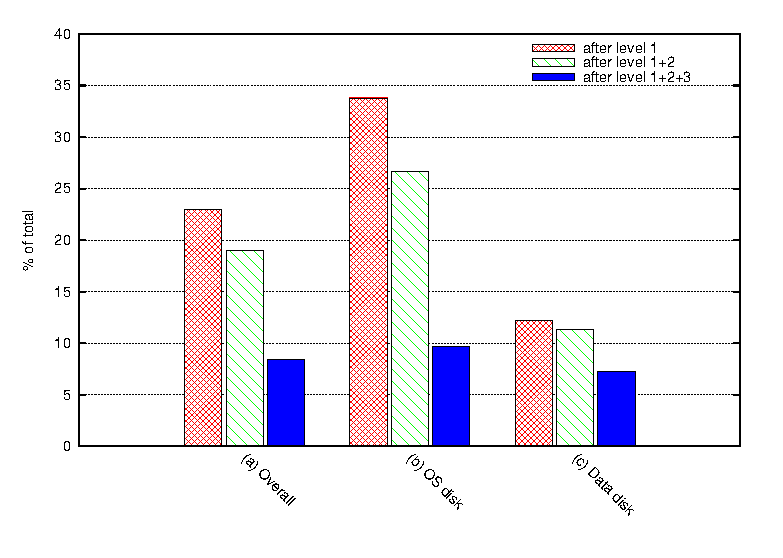
\epsfig{file=images/overall_effect.eps, width=3.5in}
%  \caption{Impacts of 3-level deduplication. The height of each bar is the data size after 
%deduplication divided by the original data size and the unit is percentage. }
%
%  \label{fig:overall}
%\end{figure}


\begin{table}[hbt]
\caption{ Performance of multi-phase deduplication.}
\begin{center}
\begin{tabular} {|c|c|c|c|c|c|}
\hline \#Partitions  & 50 & 275  &450 &  750 &  1500 \\
\hline Index+request & 161&  29 & 17.9 & 10.7 & 5.3 \\
  (MB)           &  &   &  & &  \\

\hline Time (hrs) & N/A&  3.27 & 3.09 & 3.18 & 3.42 \\
%\hline Throughput/node & N/A&  85MB/s& 90M & 87 & 81 \\
\hline Throughput GB/s& N/A&  8.5& 9 & 8.7 & 8.1 \\
\hline Option 2 time & N/A&  8& 13.3 & 18.7 & 34 \\
\hline
\end{tabular}
\end{center}
\label{tab:overall}
\end{table}

%\begin{verbatim}
%memory
%#partitions/node	50	100	250	275	300	450	500	750	1500	2000
%Memory meta data 0.161	0.0805	0.0322	0.029272727	0.026833333	0.017888889	0.0161	0.010733333	0.005366667	0.004025
%Global index 0.115	0.0575	0.023	0.020909091	0.019166667	0.012777778	0.0115	0.007666667	0.003833333	0.002875
%Seek (Step 1) 0.0212962960.0425 0.106 0.117 0.127777778	0.191666667	0.212962963	0.319444444	0.638888889	0.851851852
%Seek Option 2: 6.388888889	12.77777778	31.94444444	35.13888889	38.33333333	57.5	63.88888889	95.83333333	191.6666667	255.5555556
%Total time 3.059031718	3.078670034	3.131061779	3.137163671	3.141047877	3.313871832	3.296994302	3.377385758	3.689876824	3.901831421
%throughput  per node 0.090805785	0.090226551	0.088716799	0.088544242	0.088434748	0.083822728	0.084251822	0.082246387	0.075281044	0.07119164
%
%\end{verbatim}

The total local disk space usage for each machine is 8.05GB:  5.75GB for global index partitions and 2.3GB for accumulated requests.
Table~\ref{tab:overall} shows memory usage and performance when 
the number of parititons per machine ($q$) varies from 50 to 1500.
Row 2 shows the memory usage needed to load a partition of global index and detection requests,
varying from 161MB to 5.35MB. As we impose a constraint of 30MB, then $q=50$ would not be a viable choice.
%Row 3 shows the major  memory usage is for global index.
Row 3 is the parallel time which includes the first scanning time, 
of dirty VM segments to generate block fingerprints, data redistribution for request accumulation,
fingerprint comparison, duplicate summary distribution, and the second scan time for real backup.
Row 4 is  the aggregated throughput of  100 nodes, which is  
the size of 2500 VM images divided by the parallel time. 
Row 5 is  the aggregated throughput of  100 nodes, which is  the size of 2500 VM images divided by the parallel time. 
The result shows the backup with multi-phase deduplication  for all VM images can be completed in about 3.09 hours
with the very small resource usage.
Row 6 is  the parallel time if  we use Option 2 with $p\times q$ send buffers described in Section~\ref{sect:arch}. 
With the large number of buffers, the available space per buffer reduces significantly as $q$ increases, which leads to
a big increase of IO requests and seek cost.  


%\begin{figure}
%  \centering

%  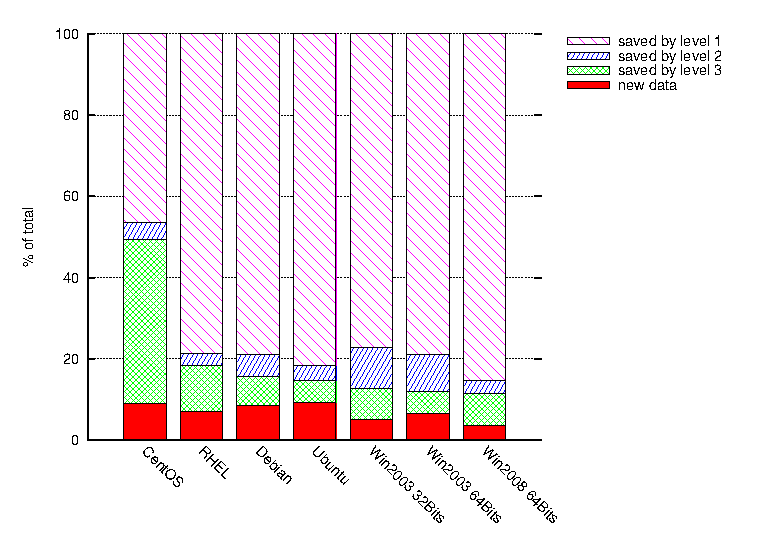
\epsfig{file=images/3level_os.eps, width=3.5in}
%  \caption{Impact of 3-level deduplication for OS releases.}
%  \label{fig:oscds}
%\end{figure}

%To see the impact of multi-level deduplication on different OS releases,
%Some of  OS disks are modified frequently and in some cases,  users even store a large amount of user data on


%\begin{verbatim}
%q= is chosen between 500 or 100
%Memory limit:   20 30M   50M  75M  100M  200M
%Time:          3.2  3.11   3  2.99 2.96  2.95
%Time for two scans: 2.78 2.78 2.78 2.78 2.78
%\end{verbatim}

\begin{figure}
\centering
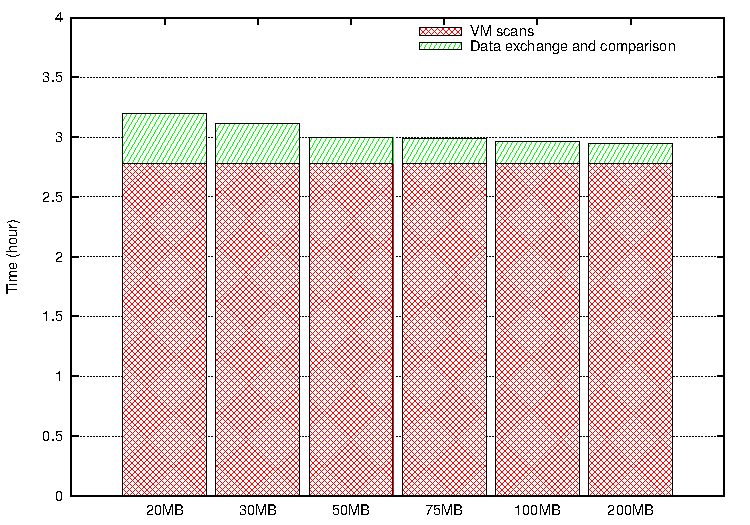
\includegraphics[width=0.4\textwidth]{mem_time.pdf}
\caption{ Parallel time when memory limit varies.}
\label{fig:memory}
\end{figure}

Figure~\ref{fig:memory} shows the performance data when 
the memory limit imposed on each node varies  from 20MB to 200MB.
The overall processing time does not have a significant reduction as we increase to 200MB.
As Row 2 shows, the time is mainly dominated by  the two scans of dirty VM segments.
Each scan takes about 1.4 hours.
Using about 30MB is sufficient to have VM backup completed in parallel 
within about 3.09 hours.

%Combining OS disks in all the VMs, we see the overall 7.4TB of data is reduced to 512GB. 
%The extreme binning approach can reduce this data set to 542GB, which is slightly worse. As a reference, 
%perfect deduplication achieves 364GB in this experiment.

%Overall speaking, inner   VM deduplication or  CDS-based deduplication
%can work well alone, but by combining them together we get a fairly good and stable deduplication ratio to 
%all kind of OSes. 
%Compared to a traditional dirty bit approach based on pages of
%each file (e.g. segment in our scheme),
%our CDS-based level 3 approach  can save additional 50\% storage space because many of level 2 block
%content can be eliminated using the CDS also.

We have also compared our multi-phase detection approach with an inline approach by combining
dirtybit segment  detection and  the data domain method~\cite{bottleneck08}. 
The bloomer filter setting  results a 1:10 ratio of index reduction for in-memory search before visiting
the disk for the full index with 2\% false positives. The prefetching cache hit ratio is set to be 98.96\% based
a number in ~\cite{bottleneck08}.
We measure its  total time including one scan of VM dirty segments in about 1.38 hours.
That approach takes about 3.19 hours comparable with our scheme while its memory takes
over 1GB for bloom filters and prefetch cache. That is an significant amount of space,
competing with other cloud service while memory cost of our setting is  insignificant.
 
%Our actual cache hit ratio tested is close 90\%.
